\documentclass[a4paper]{article}
\usepackage{geometry}
\usepackage{graphicx}
\usepackage{natbib}
\usepackage{amsmath}
\usepackage{amssymb}
\usepackage{amsthm}
\usepackage{paralist}
\usepackage{epstopdf}
\usepackage{tabularx}
\usepackage{longtable}
\usepackage{multirow}
\usepackage{multicol}
\usepackage[hidelinks]{hyperref}
\usepackage{fancyvrb}
\usepackage{algorithm}
\usepackage{algorithmic}
\usepackage{float}
\usepackage{paralist}
\usepackage[svgname]{xcolor}
\usepackage{enumerate}
\usepackage{array}
\usepackage{times}
\usepackage{url}
\usepackage{fancyhdr}
\usepackage{comment}
\usepackage{environ}
\usepackage{times}
\usepackage{textcomp}
\usepackage{caption}
\usepackage{multirow}
\usepackage{bbm}

% \usepackage{kky}

\newcounter{thm}
\ifx\fact\undefined
\newtheorem{fact}[thm]{Fact}
\fi

\newcommand{\pen}{{\rm pen}}
\newcommand{\diag}{{\rm diag}}
\newcommand{\diam}{{\bf{\rm diam}}}
\newcommand{\spann}{{\bf{\rm span}}}
\newcommand{\nulll}{{\bf{\rm null}}}
% Distributions
\newcommand{\Bern}{{\bf{\rm Bern}}\,} % support of a function
\newcommand{\Categ}{{\bf{\rm Categ}}\,} % support of a function
\newcommand{\Mult}{{\bf{\rm Mult}}\,} % support of a function
\newcommand{\Dir}{{\bf{\rm Dir}}\,} % support of a function
\newcommand{\horizontalline}{\noindent\rule[0.5ex]{\linewidth}{1pt}}
\newcommand{\HRule}{\rule{\linewidth}{0.5mm}} 
\newcommand{\Hrule}{\rule{\linewidth}{0.3mm}}
\newcommand{\HRuleN}{\HRule\\} 
\newcommand{\HruleN}{\Hrule\\}
\newcommand{\superscript}[1]{{\scriptsize \ensuremath{^{\textrm{#1}}}}}
\newcommand{\supindex}[2]{#1^{(#2)}}
\newcommand{\xii}[1]{\supindex{x}{#1}}
\newcommand{\yii}[1]{\supindex{y}{#1}}
\newcommand{\zii}[1]{\supindex{z}{#1}}
\newcommand{\Xii}[1]{\supindex{X}{#1}}
\newcommand{\Yii}[1]{\supindex{Y}{#1}}
\newcommand{\Zii}[1]{\supindex{Z}{#1}}
\newcommand{\NN}{\mathbb{N}} % Natural numbers
\newcommand{\Ncal}{\mathcal{N}}
\newcommand{\Dcal}{\mathcal{D}}
\newcommand{\Lcal}{\mathcal{L}}
\newcommand{\Xcal}{\mathcal{X}}
\newcommand{\Pcal}{\mathcal{P}}
\newcommand{\Jcal}{\mathcal{J}}
\newcommand{\Rcal}{\mathcal{R}}
\newcommand{\indfone}{\mathbbm{1}}
\newcommand{\gb}{\mathbf{g}}
\newcommand{\Hb}{\mathbf{H}}
\newcommand{\Db}{\mathbf{D}}
\newcommand*{\zero}{{\bf 0}}
\newcommand*{\one}{{\bf 1}}

% Stuff mostly appearing in Statistics
\newcommand{\Xbar}{\bar{X}}
\newcommand{\Ybar}{\bar{Y}}
\newcommand{\Zbar}{\bar{Z}}
\newcommand{\Xb}{\mathbf{X}}


%%%%  brackets
\newcommand{\inner}[2]{\left\langle #1,#2 \right\rangle}
\newcommand{\rbr}[1]{\left(#1\right)}
\newcommand{\sbr}[1]{\left[#1\right]}
\newcommand{\cbr}[1]{\left\{#1\right\}}
\newcommand{\nbr}[1]{\left\|#1\right\|}
\newcommand{\abr}[1]{\left|#1\right|}

% derivatives and partial fractions
\newcommand{\differentiate}[2]{ \frac{ \ud #2}{\ud #1} }
\newcommand{\differentiateat}[3]{ \frac{ \ud #2}{\ud #1}  \Big|_{#1=#3} }
\newcommand{\partialfrac}[2]{ \frac{ \partial #2}{\partial #1} }
\newcommand{\partialfracat}[3]{ \frac{ \partial #2}{\partial #1} \Big|_{#1=#3} }
\newcommand{\partialfracorder}[3]{ \frac{ \partial^{#3} #2}{\partial^{#3} #1} }
\newcommand{\partialfracatorder}[4]{ \frac{ \partial^{#3} #2}{\partial^{#3} #1} \Big|_{#1=#4} }

\urlstyle{rm}

\setlength\parindent{0pt} % Removes all indentation from paragraphs
\theoremstyle{definition}
\newtheorem{definition}{Definition}[]
\newtheorem{conjecture}{Conjecture}[]
\newtheorem{example}{Example}[]
\newtheorem{theorem}{Theorem}[]
\newtheorem{lemma}{Lemma}
\newtheorem{proposition}{Proposition}
\newtheorem{corollary}{Corollary}


\floatname{algorithm}{Procedure}
\renewcommand{\algorithmicrequire}{\textbf{Input:}}
\renewcommand{\algorithmicensure}{\textbf{Output:}}
\newcommand{\abs}[1]{\lvert#1\rvert}
\newcommand{\norm}[1]{\lVert#1\rVert}
\newcommand{\RR}{\mathbb{R}}
\newcommand{\EE}{\mathbb{E}}
\newcommand{\PP}{\mathbb{P}}
\newcommand{\CC}{\mathbb{C}}
\newcommand{\Nat}{\mathbb{N}}
\newcommand{\br}[1]{\{#1\}}
\DeclareMathOperator*{\argmin}{arg\,min}
\DeclareMathOperator*{\argmax}{arg\,max}
\renewcommand{\qedsymbol}{$\blacksquare$}

\definecolor{dkgreen}{rgb}{0,0.6,0}
\definecolor{gray}{rgb}{0.5,0.5,0.5}
\definecolor{mauve}{rgb}{0.58,0,0.82}

\newcommand{\Var}{\mathrm{Var}}
\newcommand{\Cov}{\mathrm{Cov}}

\newcommand{\vc}[1]{\boldsymbol{#1}}
\newcommand{\xv}{\vc{x}}
\newcommand{\Sigmav}{\vc{\Sigma}}
\newcommand{\alphav}{\vc{\alpha}}
\newcommand{\muv}{\vc{\mu}}

\newcommand{\red}[1]{\textcolor{red}{#1}}

\def\x{\mathbf x}
\def\y{\mathbf y}
\def\w{\mathbf w}
\def\v{\mathbf v}
\def\E{\mathbb E}
\def\V{\mathbb V}

\newenvironment{soln}{
    \leavevmode\color{blue}\ignorespaces
}{}



\hypersetup{
%    colorlinks,
    linkcolor={red!50!black},
    citecolor={blue!50!black},
    urlcolor={blue!80!black}
}

\geometry{
  top=1in,            % <-- you want to adjust this
  inner=1in,
  outer=1in,
  bottom=1in,
  headheight=3em,       % <-- and this
  headsep=2em,          % <-- and this
  footskip=3em,
}


\pagestyle{fancyplain}
\lhead{\fancyplain{}{Homework 5}}
\rhead{\fancyplain{}{CS 760 Machine Learning}}
\cfoot{\thepage}

\title{\textsc{Homework 5}} % Title

%%% NOTE:  Replace 'NAME HERE' etc., and delete any "\red{}" wrappers (so it won't show up as red)

\author{Dario Placencio - 907 284 6018}

\date{}

\begin{document}

\maketitle 

\textbf{Instructions:}
Use this latex file as a template to develop your homework. Submit your homework on time as a single pdf file. Please wrap your code and upload to a public GitHub repo, then attach the link below the instructions so that we can access it. Answers to the questions that are not within the pdf are not accepted. This includes external links or answers attached to the code implementation. Late submissions may not be accepted. You can choose any programming language (i.e. python, R, or MATLAB). Please check Piazza for updates about the homework. It is ok to share the experiments results and compare them with each other.

\vspace{0.1in}

\begin{soln}
    \url{github.com/placenciohid/ECE760-Homework/blob/7d85d1f10513b5c067245046def39fc576b86cde/Homework%205/HW5%20-%20Code%20-%20Dario%20Placencio.ipynb} 
\end{soln}

\section{Clustering}
\subsection{K-means Clustering (14 points)}
\begin{enumerate}

\item \textbf{(6 Points)}
Given $n$ observations $X_1^n = \{X_1, \dots, X_n\}$, $X_i \in \Xcal$, the K-means objective
is to find $k$
($<n$) centres $\mu_1^k = \{\mu_1, \dots, \mu_k\}$, and a rule $f:\Xcal \rightarrow
\{1,\dots, K\}$ so as to minimize the objective

\begin{equation}
J(\mu_1^K, f; X_1^n) = \sum_{i=1}^n \sum_{k=1}^K \indfone(f(X_i) = k) \|X_i - \mu_k\|^2
\label{eqn:kmeans}
\end{equation}

Let $\Jcal_K(X_1^n) = \min_{\mu_1^K, f} J(\mu_1^K, f; X_1^n)$. Prove that
$\Jcal_{K}(X_1^n)$ is a non-increasing function of $K$.\\

\begin{soln}
We want to show that for any given set of observations \(X_1^n\), the K-means objective function:

\[
\Jcal_{K}(X_1^n) = \min_{\mu_1^K, f} \sum_{i=1}^n \sum_{k=1}^K \mathbf{1}(f(X_i) = k) \|X_i - \mu_k\|^2
\]

is non-increasing with respect to \(K\). This means that:

\[
\Jcal_{K+1}(X_1^n) \leq \Jcal_{K}(X_1^n)
\]

Proof:

\begin{enumerate}
    \item Consider the optimal clustering given by \(\mu_1^K\) and \(f\) for \(K\) clusters that achieves the minimum in \(\Jcal_{K}(X_1^n)\).
    \item When we move from \(K\) to \(K+1\) clusters, we have two cases for the new set of centers \(\mu_1^{K+1}\):
    \begin{enumerate}
        \item The new center \(\mu_{K+1}\) is equal to one of the existing centers, say \(\mu_k\). In this case, the assignment function \(f\) can remain the same, and the objective function does not change:
        \[
        J(\mu_1^{K+1}, f; X_1^n) = J(\mu_1^K, f; X_1^n) = \Jcal_{K}(X_1^n)
        \]
        \item The new center \(\mu_{K+1}\) is different from all existing centers. In this case, at least one observation \(X_i\) that was assigned to some cluster \(k\) might now be closer to \(\mu_{K+1}\), and hence the assignment function \(f\) could change for some \(i\), possibly reducing the overall objective function. Thus:
        \[
        J(\mu_1^{K+1}, f; X_1^n) \leq J(\mu_1^K, f; X_1^n) = \Jcal_{K}(X_1^n)
        \]
    \end{enumerate}
    \item Hence, in either case, we have:
    \[
    \Jcal_{K+1}(X_1^n) \leq \Jcal_{K}(X_1^n)
    \]
\end{enumerate}

Therefore, \(\Jcal_{K}(X_1^n)\) is a non-increasing function of \(K\).
\end{soln}

\item \textbf{(8 Points)}
Consider the K-means (Lloyd's) clustering algorithm we studied in class. We
terminate the algorithm when there are no changes to the objective.
Show that the algorithm terminates in a finite number of steps.

\begin{soln}
\begin{aligned}
& \text{Let } J^{(t)} \text{ be the objective function value at iteration } t. \text{Then, } J^{(t+1)} \leq J^{(t)}. \\
& \text{At each iteration, two steps are performed:} \\
& \quad (1) \text{Cluster Assignment Step: Assign each data point } X_i \text{ to the nearest center } \mu_k. \\
& \quad (2) \text{Centroid Update Step: Update each } \mu_k \text{ to be the mean of all points assigned to cluster } k. \\
& \text{Since the mean minimizes the sum of squared distances:} \\
& \quad J^{(t+1)} = \sum_{i=1}^n \sum_{k=1}^K \mathbf{1}(f^{(t+1)}(X_i) = k) \|X_i - \mu_k^{(t+1)}\|^2 \\
& \quad \quad \quad \leq \sum_{i=1}^n \sum_{k=1}^K \mathbf{1}(f^{(t)}(X_i) = k) \|X_i - \mu_k^{(t)}\|^2 = J^{(t)}. \\
& \text{Since there are a finite number of data points, there are a finite number of possible assignments of points to } K \text{ clusters.} \\
& \text{Thus, the algorithm must terminate in a finite number of steps as the objective function } J \text{ cannot decrease indefinitely.}
\end{aligned}
\end{soln}

\end{enumerate}

\subsection{Experiment (20 Points)}

In this question, we will evaluate
K-means clustering and GMM on a simple 2 dimensional problem.
First, create a two-dimensional synthetic dataset of 300 points by sampling 100 points each from the
three Gaussian distributions shown below:
\[
P_a = \Ncal\left(
\begin{bmatrix}
-1 \\ -1
\end{bmatrix},
\;
\sigma\begin{bmatrix}
2, &0.5 \\ 0.5, &1
\end{bmatrix}
\right),
\quad
P_b = \Ncal\left(
\begin{bmatrix}
1 \\ -1
\end{bmatrix},
\;
 \sigma\begin{bmatrix}
1, &-0.5 \\ -0.5, &2
\end{bmatrix}
\right),
\quad
P_c = \Ncal\left(
\begin{bmatrix}
0 \\ 1
\end{bmatrix},
\;
 \sigma\begin{bmatrix}
1 &0 \\ 0, &2
\end{bmatrix}
\right)
\]
Here, $\sigma$ is a parameter we will change to produce different datasets.\\

First implement K-means clustering and the expectation maximization algorithm for GMMs.
Execute both methods on five synthetic datasets,
generated as shown above with $\sigma \in \{0.5, 1, 2, 4, 8\}$. Finally, evaluate both methods on \emph{(i)} the clustering objective~\eqref{eqn:kmeans} and \emph{(ii)}  the clustering accuracy. For each of the two criteria, plot the value achieved by each method against $\sigma$.\\


Guidelines:
\begin{itemize} 
\item Both algorithms are only guaranteed to find only a local optimum so we recommend trying multiple
restarts and picking the one with the lowest objective value (This is~\eqref{eqn:kmeans} for K-means and the negative log likelihood for GMMs).
You may also experiment with a smart initialization
strategy (such as kmeans++).

\item
To plot the clustering accuracy,  you may treat the `label' of points generated from distribution
$P_u$ as $u$, where $u\in \{a, b, c\}$.
Assume that the cluster id $i$ returned by a method is $i\in \{1, 2, 3\}$.
Since clustering is an unsupervised learning problem, you should obtain the best possible mapping
from $\{1, 2, 3\}$ to $\{a, b, c\}$ to compute the clustering objective.
One way to do this is to compare the clustering centers returned by the method (centroids for
K-means, means for GMMs) and map them to the distribution with the closest mean.

\end{itemize}

Points break down: 7 points each for implementation of each method, 6 points for reporting of
evaluation metrics.


\section{Linear Dimensionality Reduction}

\subsection{Principal Components Analysis  (10 points)}
\label{sec:pca}

Principal Components Analysis (PCA) is a popular method for linear dimensionality reduction. PCA attempts to find a lower dimensional subspace such that when you project the data onto the subspace as much of the information is preserved. Say we have data $X = [x_1^\top; \dots; x_n^\top] \in \RR^{n\times D}$ where  $x_i \in \RR^D$. We wish to find a $d$ ($ < D$) dimensional subspace $A = [a_1, \dots, a_d] \in \RR^{D\times d}$, such that $ a_i \in \RR^D$ and $A^\top A = I_d$, so as to maximize $\frac{1}{n} \sum_{i=1}^n \|A^\top x_i\|^2$.
\begin{enumerate}

\item  \textbf{(4 Points)}
Suppose we wish to find the first direction $a_1$ (such that $a_1^\top a_1 = 1$) to maximize $\frac{1}{n} \sum_i (a_1^\top x_i)^2$.
Show that $a_1$ is the first right singular vector of $X$.

\begin{soln}
Given the data matrix $X \in \mathbb{R}^{n \times D}$, we want to find the first principal component $a_1 \in \mathbb{R}^D$ such that $a_1^\top a_1 = 1$ and it maximizes the quantity $\frac{1}{n} \sum_{i=1}^n (a_1^\top x_i)^2$.

Using the singular value decomposition, we can write $X$ as $X = U\Sigma V^\top$, where $U \in \mathbb{R}^{n \times n}$ and $V \in \mathbb{R}^{D \times D}$ are orthogonal matrices and $\Sigma \in \mathbb{R}^{n \times D}$ is a diagonal matrix with non-negative real numbers on the diagonal.
  
The columns of $V$ (the right singular vectors) are the eigenvectors of $X^\top X$, and the columns of $U$ (the left singular vectors) are the eigenvectors of $XX^\top$.
  
The optimization problem for the first principal component can be written as:
  
  \begin{equation}
  \max_{a_1: a_1^\top a_1 = 1} \frac{1}{n} \sum_{i=1}^n (a_1^\top x_i)^2 = \max_{a_1: a_1^\top a_1 = 1} a_1^\top \left(\frac{1}{n} \sum_{i=1}^n x_i x_i^\top \right) a_1.
  \end{equation}
  
This is equivalent to the Rayleigh quotient, which is maximized when $a_1$ is the eigenvector corresponding to the largest eigenvalue of the covariance matrix $\frac{1}{n}X^\top X$.
  
Since $V$ contains the eigenvectors of $X^\top X$, the first column of $V$, which corresponds to the largest singular value (and thus the largest eigenvalue of $X^\top X$), is the solution to our optimization problem. Therefore, $a_1$ is the first right singular vector of $X$.
\end{soln}

\item  \textbf{(6 Points)}
Given $a_1, \dots, a_k$, let $A_k = [a_1, \dots, a_k]$ and 
$\tilde{x}_i = x_i - A_kA_k^\top x_i$. We wish to find $a_{k+1}$, to maximize
$\frac{1}{n} \sum_i (a_{k+1}^\top \tilde{x}_i)^2$. Show that $a_{k+1}$ is the
$(k+1)^{th}$ right singular vector of $X$.

\begin{soln}
Given the data matrix \( X \in \mathbb{R}^{n \times D} \), suppose we have already found the first \( k \) principal components \( a_1, \dots, a_k \) and constructed the matrix \( A_k = [a_1, \dots, a_k] \). For each data point \( x_i \), we define the residual after projecting onto the subspace spanned by \( A_k \) as \( \tilde{x}_i = x_i - A_kA_k^\top x_i \). We wish to find the next principal component \( a_{k+1} \) such that it maximizes the variance of the residuals, i.e.,

\begin{equation}
\max_{a_{k+1}: a_{k+1}^\top a_{k+1} = 1} \frac{1}{n} \sum_{i=1}^n (a_{k+1}^\top \tilde{x}_i)^2.
\end{equation}
  
This is equivalent to finding the eigenvector associated with the largest eigenvalue of the covariance matrix of the residuals, \( \frac{1}{n}\tilde{X}^\top \tilde{X} \), where \( \tilde{X} \) is the matrix with rows \( \tilde{x}_i^\top \).
  
Note that \( \tilde{X} \) can be written as \( \tilde{X} = X - A_kA_k^\top X \). Using the fact that \( A_k \) is orthogonal to the residual space and \( A_k^\top A_k = I_k \), we can perform an SVD on \( \tilde{X} \) to find its right singular vectors.
  
The \((k+1)^{th}\) principal component \( a_{k+1} \) will then be the right singular vector of \( \tilde{X} \) associated with its largest singular value, which is not in the span of \( A_k \). Since the singular vectors of \( \tilde{X} \) and \( X \) are the same beyond the first \( k \) vectors, \( a_{k+1} \) is also the \((k+1)^{th}\) right singular vector of \( X \).
 
Thus, we conclude that \( a_{k+1} \) is the \((k+1)^{th}\) right singular vector of \( X \).
\end{soln}

\end{enumerate}

\subsection{Dimensionality reduction via optimization (22 points)}

We will now motivate the dimensionality reduction problem from a slightly different
perspective. The resulting algorithm has many similarities to PCA.
We will refer to method as DRO.

As before, you are given data $\{x_i\}_{i=1}^n$, where $x_i \in \RR^D$. Let $X=[x_1^\top; \dots
x_n^\top] \in \RR^{n\times D}$. We suspect that the data
actually lies approximately in  a $d$ dimensional affine subspace.
Here $d<D$ and $d<n$.
Our goal, as in PCA, is to use this dataset to find a $d$ dimensional representation $z$ for each $x\in\RR^D$.
(We will assume that the span of the data has dimension larger than
$d$, but our method should work whether $n>D$ or $n<D$.)


Let $z_i\in \RR^d$ be the lower dimensional representation for $x_i$ and
let $Z = [z_1^\top; \dots; z_n^\top] \in \RR^{n\times d}$.
We wish to find parameters $A \in \RR^{D\times d}$, $b\in\RR^D$ and the lower
dimensional representation $Z\in \RR^{n\times d}$ so as to minimize 
\begin{equation}
J(A,b,Z) = \frac{1}{n} \sum_{i=1}^n \|x_i - Az_i - b\|^2 = \| X - ZA^\top - \one b^\top\|_F^2.
\label{eqn:dimobj}
\end{equation}
Here, $\|A\|^2_F = \sum_{i,j} A_{ij}^2$ is the Frobenius norm of a matrix.


\begin{enumerate}
\item \textbf{(3 Points)}
Let $M\in\RR^{d\times d}$ be an arbitrary invertible matrix and $p\in\RR^{d}$ be an arbitrary vector.
Denote, $A_2 = A_1M^{-1}$, $b_2 = b_1- A_1M^{-1}p$ and $Z_2 = Z_1 M^\top +
\one p^\top$.
Show that both
$(A_1, b_1, Z_1)$ and $(A_2, b_2, Z_2)$ achieve the same objective value $J$~\eqref{eqn:dimobj}.
\end{enumerate}

Therefore, in order to make the problem determined, we need to impose some
constraint on $Z$. We will assume that the $z_i$'s have zero mean and identity covariance.
That is,
\begin{align*}
\Zbar = \frac{1}{n} \sum_{i=1}^n z_i =\frac{1}{n} Z^\top {\bf 1}_n = 0, \hspace{0.3in} 
S = \frac{1}{n} \sum_{i=1}^n z_i z_i^\top 
= \frac{1}{n} Z^\top Z
= I_d
\end{align*}
Here, ${\bf 1}_d = [1, 1 \dots, 1]^\top \in\RR^d$ and $I_d$  is the $d\times d$ identity matrix.\\


\begin{soln}
To show that both \((A_1, b_1, Z_1)\) and \((A_2, b_2, Z_2)\) achieve the same objective value \(J\), we must demonstrate that the transformation involving \(M\) and \(p\) does not change the Frobenius norm of the error matrix.
    
    Let's consider the transformed variables:
    
    \begin{align*}
    A_2 &= A_1M^{-1}, \\
    b_2 &= b_1 - A_1M^{-1}p, \\
    Z_2 &= Z_1 M^\top + \mathbf{1} p^\top.
    \end{align*}
    
    The objective function \(J(A, b, Z)\) is defined as:
    
    \[
    J(A, b, Z) = \frac{1}{n} \sum_{i=1}^n \|x_i - A z_i - b\|^2 = \| X - Z A^\top - \mathbf{1} b^\top \|_F^2.
    \]
    
    Now, we substitute \(A_2\), \(b_2\), and \(Z_2\) into the objective function and simplify:
        
    \begin{align*}
    J(A_2, b_2, Z_2) &= \| X - Z_2A_2^\top - \mathbf{1} b_2^\top\|_F^2 \\
    &= \| X - (Z_1 M^\top + \mathbf{1} p^\top)(M^{-1})^\top A_1^\top - \mathbf{1} (b_1 - A_1M^{-1}p)^\top\|_F^2 \\
    &= \| X - Z_1 A_1^\top - \mathbf{1} p^\top A_1^\top - \mathbf{1} b_1^\top + \mathbf{1} p^\top A_1^\top \|_F^2 \\
    &= \| (X - Z_1 A_1^\top - \mathbf{1} b_1^\top) + \mathbf{1} p^\top A_1^\top - \mathbf{1} p^\top A_1^\top \|_F^2 \\
    &= \| X - Z_1 A_1^\top - \mathbf{1} b_1^\top \|_F^2 \\
    &= J(A_1, b_1, Z_1).
    \end{align*}
    
    Thus, the objective value remains unchanged under the transformation using \(M\) and \(p\), showing that \(J(A_1, b_1, Z_1) = J(A_2, b_2, Z_2)\). This means that the solution is not unique and that any set of parameters related by an invertible linear transformation will yield the same objective value. Therefore, constraints must be imposed on \(Z\) to make the problem well-defined, such as requiring that \(Z\) has zero mean and identity covariance.
\end{soln}

\begin{enumerate}
\setcounter{enumi}{1}
\item \textbf{(16 Points)}
Outline a procedure to solve the above problem. Specify how you
would obtain $A, Z, b$ which minimize the objective and satisfy the constraints.

\textbf{Hint: }The rank $k$ approximation of a matrix in Frobenius norm is obtained by
taking its SVD and then zeroing out all but the first $k$ singular values.

\begin{soln}
To solve the given problem, we can leverage the fact that the best rank \( k \) approximation in the Frobenius norm of a matrix is given by its Singular Value Decomposition (SVD) truncated to the first \( k \) singular values. The optimization process can be outlined as follows:

1. Center the Data: Subtract the mean of the data points from each point to ensure that the data is centered around the origin. Let \( \bar{x} \) be the mean of \( \{x_i\}_{i=1}^n \), then we update \( x_i \) to \( x_i - \bar{x} \) for each \( i \). This centers \( X \) and allows us to ignore \( b \) in the initial steps since it's now zero.
    
2. SVD of the Centered Data: Compute the SVD of the centered data matrix \( X \). The SVD is given by \( X = U\Sigma V^\top \), where \( U \) and \( V \) are orthogonal matrices, and \( \Sigma \) is a diagonal matrix with non-negative real numbers on the diagonal (singular values).
    
3. Truncate the SVD: To get a rank \( d \) approximation of \( X \), retain only the first \( d \) columns of \( U \) and \( V \), and the first \( d \) singular values in \( \Sigma \). This gives the matrices \( U_d \), \( \Sigma_d \), and \( V_d \).
    
4. Compute the Lower Dimensional Representation \( Z \): The matrix \( Z \) can be computed as \( Z = U_d \Sigma_d \). This is the projection of the data onto the \( d \)-dimensional subspace that captures the most variance.
    
5. Reconstruct \( A \): The matrix \( A \) can be computed as the first \( d \) columns of \( V \) (i.e., \( V_d \)).
    
6. Recover \( b \): Now that we have \( Z \) and \( A \), we can find \( b \) by solving the equation \( \bar{x} = A\bar{z} + b \), where \( \bar{z} \) is the mean of the projections \( Z \). Since \( Z \) has zero mean by construction, \( b \) is simply the original mean \( \bar{x} \) of the data.
    
7. Enforce the Constraints: To ensure that \( Z \) has zero mean and identity covariance, we can further orthogonalize \( Z \) using QR decomposition if necessary. However, if the SVD is computed correctly, \( Z \) should already satisfy these constraints.
    
The procedure outlined above provides a solution to the dimensionality reduction problem as specified, yielding the parameters \( A \), \( Z \), and \( b \) that minimize the objective while satisfying the constraints of zero mean and identity covariance for \( Z \).
\end{soln}

\item \textbf{(3 Points)}
You are given a point $x_*$ in the original $D$ dimensional space.
State the rule to obtain the $d$ dimensional
representation $z_*$ for this new point.
(If $x_*$ is some original point $x_i$ from the $D$--dimensional space, it shoud be the
$d$--dimensional representation $z_i$.)

\begin{soln}
To obtain the \( d \)-dimensional representation \( z_* \) for a new point \( x_* \) in the original \( D \)-dimensional space, we could follow these steps:

1. Center the New Point: Subtract the mean \( \bar{x} \) of the original data points from \( x_* \) to center it in the same way as the original data. This gives the centered point \( x_{\text{centered}} = x_* - \bar{x} \).
    
2. Project onto the New Subspace: Use the matrix \( A \) obtained from the dimensionality reduction process to project the centered point onto the new \( d \)-dimensional subspace. This is done by calculating \( z_* = A^\top x_{\text{centered}} \).
    
The resulting vector \( z_* \) is the \( d \)-dimensional representation of \( x_* \). This representation will be consistent with the representations obtained for the original data points, meaning that if \( x_* \) was an original data point \( x_i \), then \( z_* \) should correspond to the \( d \)-dimensional representation \( z_i \) obtained during the dimensionality reduction process.
\end{soln}

\end{enumerate}


\subsection{Experiment (34 points)}

Here we will compare the above three methods on two data sets. 

\begin{itemize}
\item We will implement three variants of PCA:
\begin{enumerate}
    \item "buggy PCA": PCA applied directly on the matrix $X$.
    \item "demeaned PCA": We subtract the mean along each dimension before applying PCA.
    \item "normalized PCA": Before applying PCA, we subtract the mean and scale each dimension so that the sample  mean and standard deviation along each dimension is $0$ and $1$ respectively.
    
\end{enumerate}



\item 
One way to study how well the low dimensional representation $Z$ captures the linear
structure in our data is to project $Z$ back to $D$ dimensions and look at the reconstruction
error. For PCA, if we mapped it to $d$ dimensions via $z = Vx$ then the
reconstruction is $V^\top z$. For the preprocessed versions, we first do this and then
reverse the preprocessing steps as well. For DRO  we just compute $Az + b$.
We will compare all methods by the reconstruction error on the datasets.

\item 
Please implement code for the methods: Buggy PCA (just take the SVD of $X$)
, Demeaned PCA,
Normalized PCA, DRO. In all cases your function should take in
an $n \times d$ data matrix and $d$ as an argument. It should return the
the $d$ dimensional representations, the estimated parameters, and the
reconstructions of these representations in $D$ dimensions. 

\item
You are given two datasets: A two Dimensional dataset with $50$ points 
\texttt{data2D.csv} and a thousand dimensional dataset with $500$ points
\texttt{data1000D.csv}. 

\item
For the $2D$ dataset use $d=1$. For the $1000D$ dataset, you need to choose
$d$. For this, observe the singular values in DRO and see if there is a clear
``knee point" in the spectrum.
Attach any figures/ Statistics you computed to justify your choice.

\item
For the $2D$ dataset you need to attach the a 
plot comparing the orignal points with the reconstructed points for all 4
methods.
For both datasets you should also report the reconstruction errors, that is the squared sum of
differences $\sum_{i=1}^n \|x_i - r(z_i)\|^2$,
where $x_i$'s are the original points and $r(z_i)$ are the $D$ dimensional points
reconstructed from the 
$d$ dimensional representation $z_i$.

\item \textbf{Questions:} After you have completed the experiments, please answer the following questions.
\begin{enumerate}
\item Look at the results for Buggy PCA. The reconstruction error is bad and the
reconstructed points don't seem to well represent the original points. Why is
this? \\
\textbf{Hint: } Which subspace is Buggy PCA trying to project the points
onto?
\item The error criterion we are using is the average squared error 
between the original points and the reconstructed points.
In both examples DRO and demeaned PCA achieves the lowest error among all
methods. 
Is this surprising? Why?
\end{enumerate}

\item Point allocation:
\begin{itemize}
\item Implementation of the three PCA methods: \textbf{(6 Points)}
\item Implementation of DRO: \textbf{(6 points)}
\item Plots showing original points and reconstructed points for 2D dataset for each one of the 4 methods: \textbf{(10 points)}
\item Implementing reconstructions and reporting results for each one of the 4 methods for the 2 datasets: \textbf{(5 points)}
\item Choice of $d$ for $1000D$ dataset and appropriate justification:
\textbf{(3 Points)}
\item Questions \textbf{(4 Points)}
\end{itemize}

\end{itemize}


%\vspace{0.1in}

\vspace{0.2in}

\textbf{Answer format:}  \\
The graph bellow is in example of how a plot of one of the algorithms for the 2D dataset may look like: \\
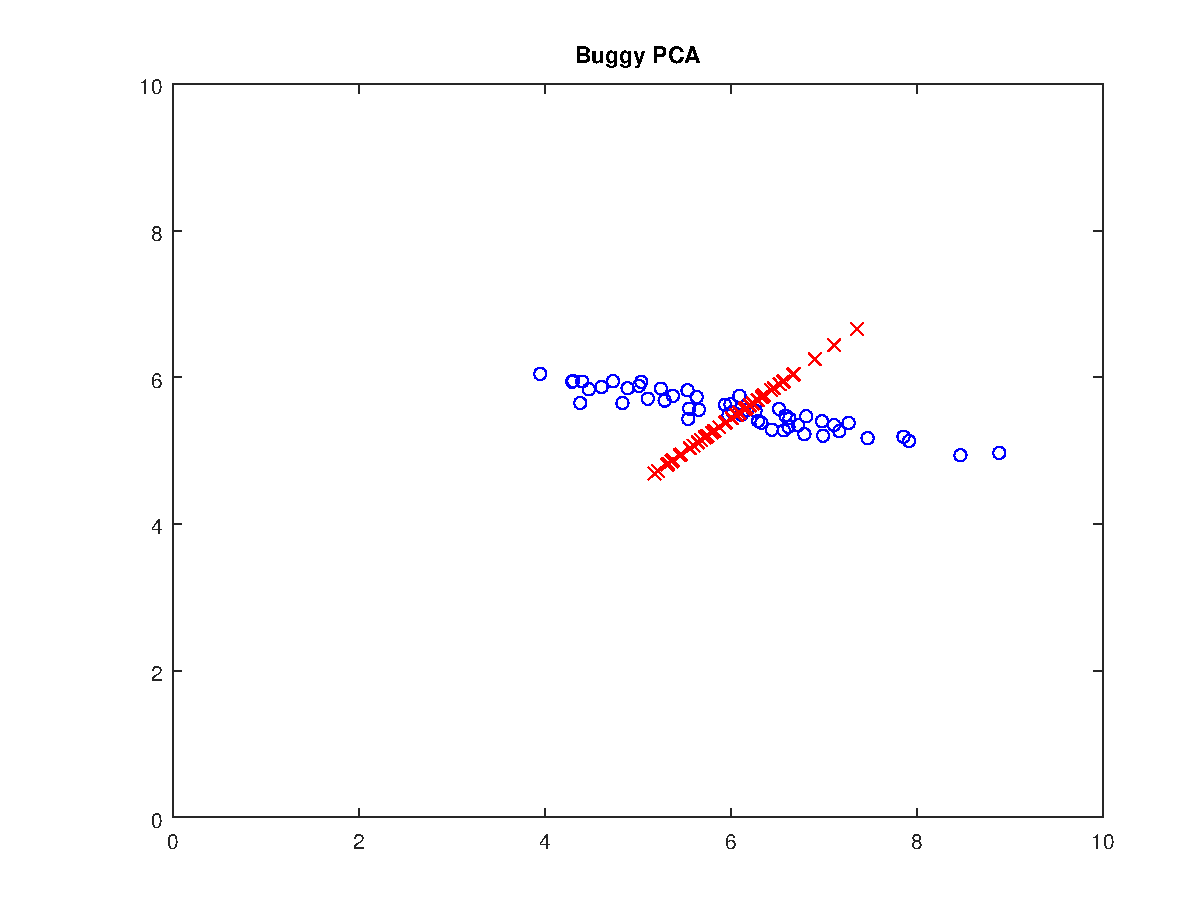
\includegraphics[width=3in]{buggy_pca} \hspace{0.4in}
\\

The blue circles are from the original dataset and the red crosses are the reconstructed points. \\

And this is how the reconstruction error may look like for Buggy PCA for the 2D dataset: 0.886903

\bibliographystyle{apalike}
\end{document}


